%IEEE TIFS For new manuscripts, the page limit is 13 pages in double-column format.

\documentclass[journal]{IEEEtran}
%,onecolumn,12pt
% If IEEEtran.cls has not been installed into the LaTeX system files,
% manually specify the path to it like:
% \documentclass[journal]{../sty/IEEEtran}


\usepackage{graphics} % for pdf, bitmapped graphics files
\usepackage{epsfig} % for postscript graphics files
\usepackage{mathptmx} %  It supersedes both the original times and the mathptm packages.
\usepackage{amsthm}
\usepackage{amsmath} % assumes amsmath package installed
\usepackage{amssymb}  % assumes amsmath package installed
\usepackage{cuted}
\usepackage{float}
\usepackage{color}
\usepackage{url}
\usepackage{bm}

\usepackage[ruled,vlined,linesnumbered]{algorithm2e} %noresetcount %use this 
\usepackage{tabularx}
\usepackage{caption}
\usepackage{subcaption}
%\usepackage[font=small]{caption}
%\renewcommand\thesubtable{(\alph{subtable})}

\newtheorem{theorem}{Theorem}
\newtheorem{corollary}{Corollary}
\newtheorem{lemma}{Lemma}
\newtheorem{proposition}{Proposition}
\newtheorem{definition}{Definition}
\newtheorem{metric}{Metric}
\newtheorem{principle}{Principle}
\newtheorem{remark}{Remark}
\newtheorem{example}{Example}


% correct bad hyphenation here
\hyphenation{op-tical net-works semi-conduc-tor}


% uncomment the following part to see a changing header
% \makeatletter %@ 现在算字母
% \def\ps@IEEEtitlepagestyle{%
%   \def\@oddfoot{\mycopyrightnotice}%
%   \def\@evenfoot{}%
% }
% \def\mycopyrightnotice{%
%   \begin{minipage}{\textwidth}
%   \centering \scriptsize
%   Copyright~\copyright~2026 IEEE. Personal use of this material is permitted. Permission from IEEE must be obtained for all other uses, in any current or future media, including reprinting/republishing this material for advertising or promotional purposes, creating new collective works, for resale or redistribution to servers or lists, or reuse of any copyrighted component of this work in other works. 
%   \end{minipage}
% }
% \makeatother %@ 不再是字母





\begin{document}
%
% paper title
% Titles are generally capitalized except for words such as a, an, and, as,
% at, but, by, for, in, nor, of, on, or, the, to and up, which are usually
% not capitalized unless they are the first or last word of the title.
% Linebreaks \\ can be used within to get better formatting as desired.
% Do not put math or special symbols in the title.
\title{
%From Cryptographic Protection to Situation-Aware Assurance: Securing Future Satellite Operations 
Beyond Cryptographic Validity: Situation-Aware Security for Future Satellite Operations
} 

\author{
Linan Huang, %~\IEEEmembership{Member,~IEEE},
Houdong Wang, 
and Linling Kuang  
\thanks{L. Huang is with the Beijing National Research Center for Information Science and Technology (BNRist), Tsinghua University, Beijing 100084, China (e-mail: huanglinan@tsinghua.edu.cn).}%
\thanks{H. Wang is with the Department of Electronic Engineering, Tsinghua University, Beijing 100084, China (e-mail: hd-wang21@mails.tsinghua.edu.cn).}% <-this % stops a space
\thanks{L. Kuang is with the Beijing National Research Center for Information Science and Technology, and the State Key Laboratory of Space Network and Communications, Tsinghua University, Beijing 100084, China (e-mail: kll@tsinghua.edu.cn).}
}


% The paper headers
\markboth{Journal of \LaTeX\ Class Files,~Vol.~14, No.~8, August~2015}%
{Shell \MakeLowercase{\textit{et al.}}: Bare Demo of IEEEtran.cls for IEEE Journals}
% The only time the second header will appear is for the odd numbered pages
% after the title page when using the twoside option.
% 
% *** Note that you probably will NOT want to include the author's ***
% *** name in the headers of peer review papers.                   ***
% You can use \ifCLASSOPTIONpeerreview for conditional compilation here if
% you desire.




% If you want to put a publisher's ID mark on the page you can do it like
% this:
%\IEEEpubid{0000--0000/00\$00.00~\copyright~2015 IEEE}
% Remember, if you use this you must call \IEEEpubidadjcol in the second
% column for its text to clear the IEEEpubid mark.



% use for special paper notices
%\IEEEspecialpapernotice{(Invited Paper)}




% make the title area
\maketitle

% As a general rule, do not put math, special symbols or citations
% in the abstract or keywords.
 %TC:ignore 
\begin{abstract}
XXXX
\end{abstract}
 %TC:endignore 

 
% Note that keywords are not normally used for peerreview papers.
% \begin{IEEEkeywords}
% Satellite Constellation, 
% \end{IEEEkeywords}

\section{Introduction} %500~800 words
\label{sec:Intro}
%系统演进趋势：网络化、多功能、自主性强
Future satellite systems are evolving from remotely commanded communication terminals into networked, multi-functional, and increasingly autonomous computing platforms. 
%趋势导致星上安全的重要性和内涵的提升：从数据保护到复杂状态下的保护
As information processing, computing, and decision-making capabilities increasingly migrate from the ground to onboard satellite systems, both the importance and the scope of onboard security are expanding accordingly. 
In addition to communication data, security mechanisms must now protect increasingly complex onboard states, processing logic, and control procedures. 

%建立基线：卫星系统各个层级的协议栈都有成熟的密码保护机制
Satellite communication systems have developed a broad range of cryptographic protection mechanisms across multiple protocol layers. Representative examples include the CCSDS Space Data Link Security Protocol \cite{ccsds2022sdls} for conventional space links and Internet security protocols (e.g., IPsec) that can be adapted to emerging IP-based integrated space--terrestrial networks \cite{ahmad2022security}. 
%基线问题：密码学有效不等于操作合法，即Cryptographic validity does not guarantee operational legitimacy
These mechanisms can authenticate message origins, ensure message integrity, and protect message confidentiality.
However, cryptographic validity alone does not guarantee operational legitimacy. 
A message may be correctly authenticated and integrity-protected, yet still be inappropriate under the current operational context. 
For example, a telemetry, tracking, and command (TT\&C) command originating from a compromised user terminal should neither be executed nor even forwarded to the onboard command and data handling computer, because a user terminal is not authorized to perform spacecraft control operations. 
%亮明观点：从CIA triad到situation-aware security
Future satellite security must extend beyond the traditional CIA triad toward situation-aware protection that evaluates the operational legitimacy of authenticated actions and safeguards the correctness, continuity, and resilience of onboard operations.

Addressing this gap gives rise to three fundamental challenges.
%Challenge 1： 在多流明密态管理等复杂安全状态需要持续维护的情况下，如何实现高可信、抗攻击的状态管理？
The first challenge lies in reconciling state complexity with trustworthiness. Future satellites need to maintain rich and evolving security states to enable resilient secure mechanisms such as clear/protected mode management and transition \cite{huang2026toward}. 
However, greater state complexity makes the management logic harder to verify and expands its attack surface. The key question is therefore how to support complex security-state evolution while keeping the security-critical state-management core trustworthy and attack-resilient. 

%Challenge 2： 在星地链路资源有限且敏感安全状态不可直接暴露的约束下，如何在地面高效、准确地重建星上安全状态？
The second challenge concerns XXXX
%ground-side awareness of onboard security states. Ground operators need sufficient knowledge of onboard state evolution to diagnose anomalies, verify transitions, and coordinate recovery actions. However, satellite–ground links provide limited telemetry capacity, while many security states—such as active keys, detailed Security Association parameters, and internal protection configurations—cannot be directly exposed without introducing additional security risks. The resulting question is how to efficiently and accurately reconstruct onboard security states from limited and non-sensitive observations.

%Challenge 3：在卫星系统日益网络化、分布式和自主化的背景下，如何充分发挥不同节点与运行环节的互补作用，对安全关键操作是否合法形成系统级判断？
The third challenge concerns system-level verification of operational legitimacy. In increasingly networked, distributed, and autonomous satellite systems, relevant evidence is often fragmented across nodes and operational stages, and may be heterogeneous, partial, or inconsistent. The key question is how to design mechanisms that actively trigger and orchestrate the systematic use of such evidence to derive reliable security knowledge and judgments, while adapting to satellite-specific architectures and stringent SWaP constraints.

%解决3个挑战的大致思路
This article aims to fill these gaps. 
%最小分离的架构（包含了规整的接口）+ 合理的对多状态的处理顺序。
To address the first challenge, we propose a minimally decoupled architecture that separates complex, mission-specific state management from a minimal and standardized cryptographic unit through well-defined control and data interfaces. On this basis, we define the responsibilities of the two units and establish a disciplined processing order for state evaluation and cryptographic execution, ensuring consistent handling of multiple interdependent security states. 

For the second challenge of XXX, we XXX. 

To address the third challenge, we adopt a role-aware strategy. Rather than burdening every node with equal security obligations—or expecting a single node to fully validate an operation alone—we distribute differentiated responsibilities among source, forwarding, destination, and execution nodes. Assignments are tailored to each node’s place in the workflow, its available context, and its practical verification capacity.

%研究内容之间的关系，结合图1的章节组织来介绍
As shown in Fig. \ref{fig:PaperStructure}, the overall structure of this paper constructs to expand traditional crypto validity to situation-aware security by solving three challenges in Section \ref{sec:point1}, \ref{sec:point2}, \ref{sec:point3}. 
%第一个challenge可以视为是传统加解密在复杂系统状态下的拓展，建立可信基础/底座。第二个和第三个challenge分别从可感知和可验证两个角度进行面向Situation-Aware的拓展。
The first can be viewed as extending conventional cryptographic processing to complex system states, thereby laying a trustworthy foundation. The second and third further advance toward situation-aware security from the perspectives of perceptibility and verifiability, respectively. 

\begin{figure}[t]
\centering
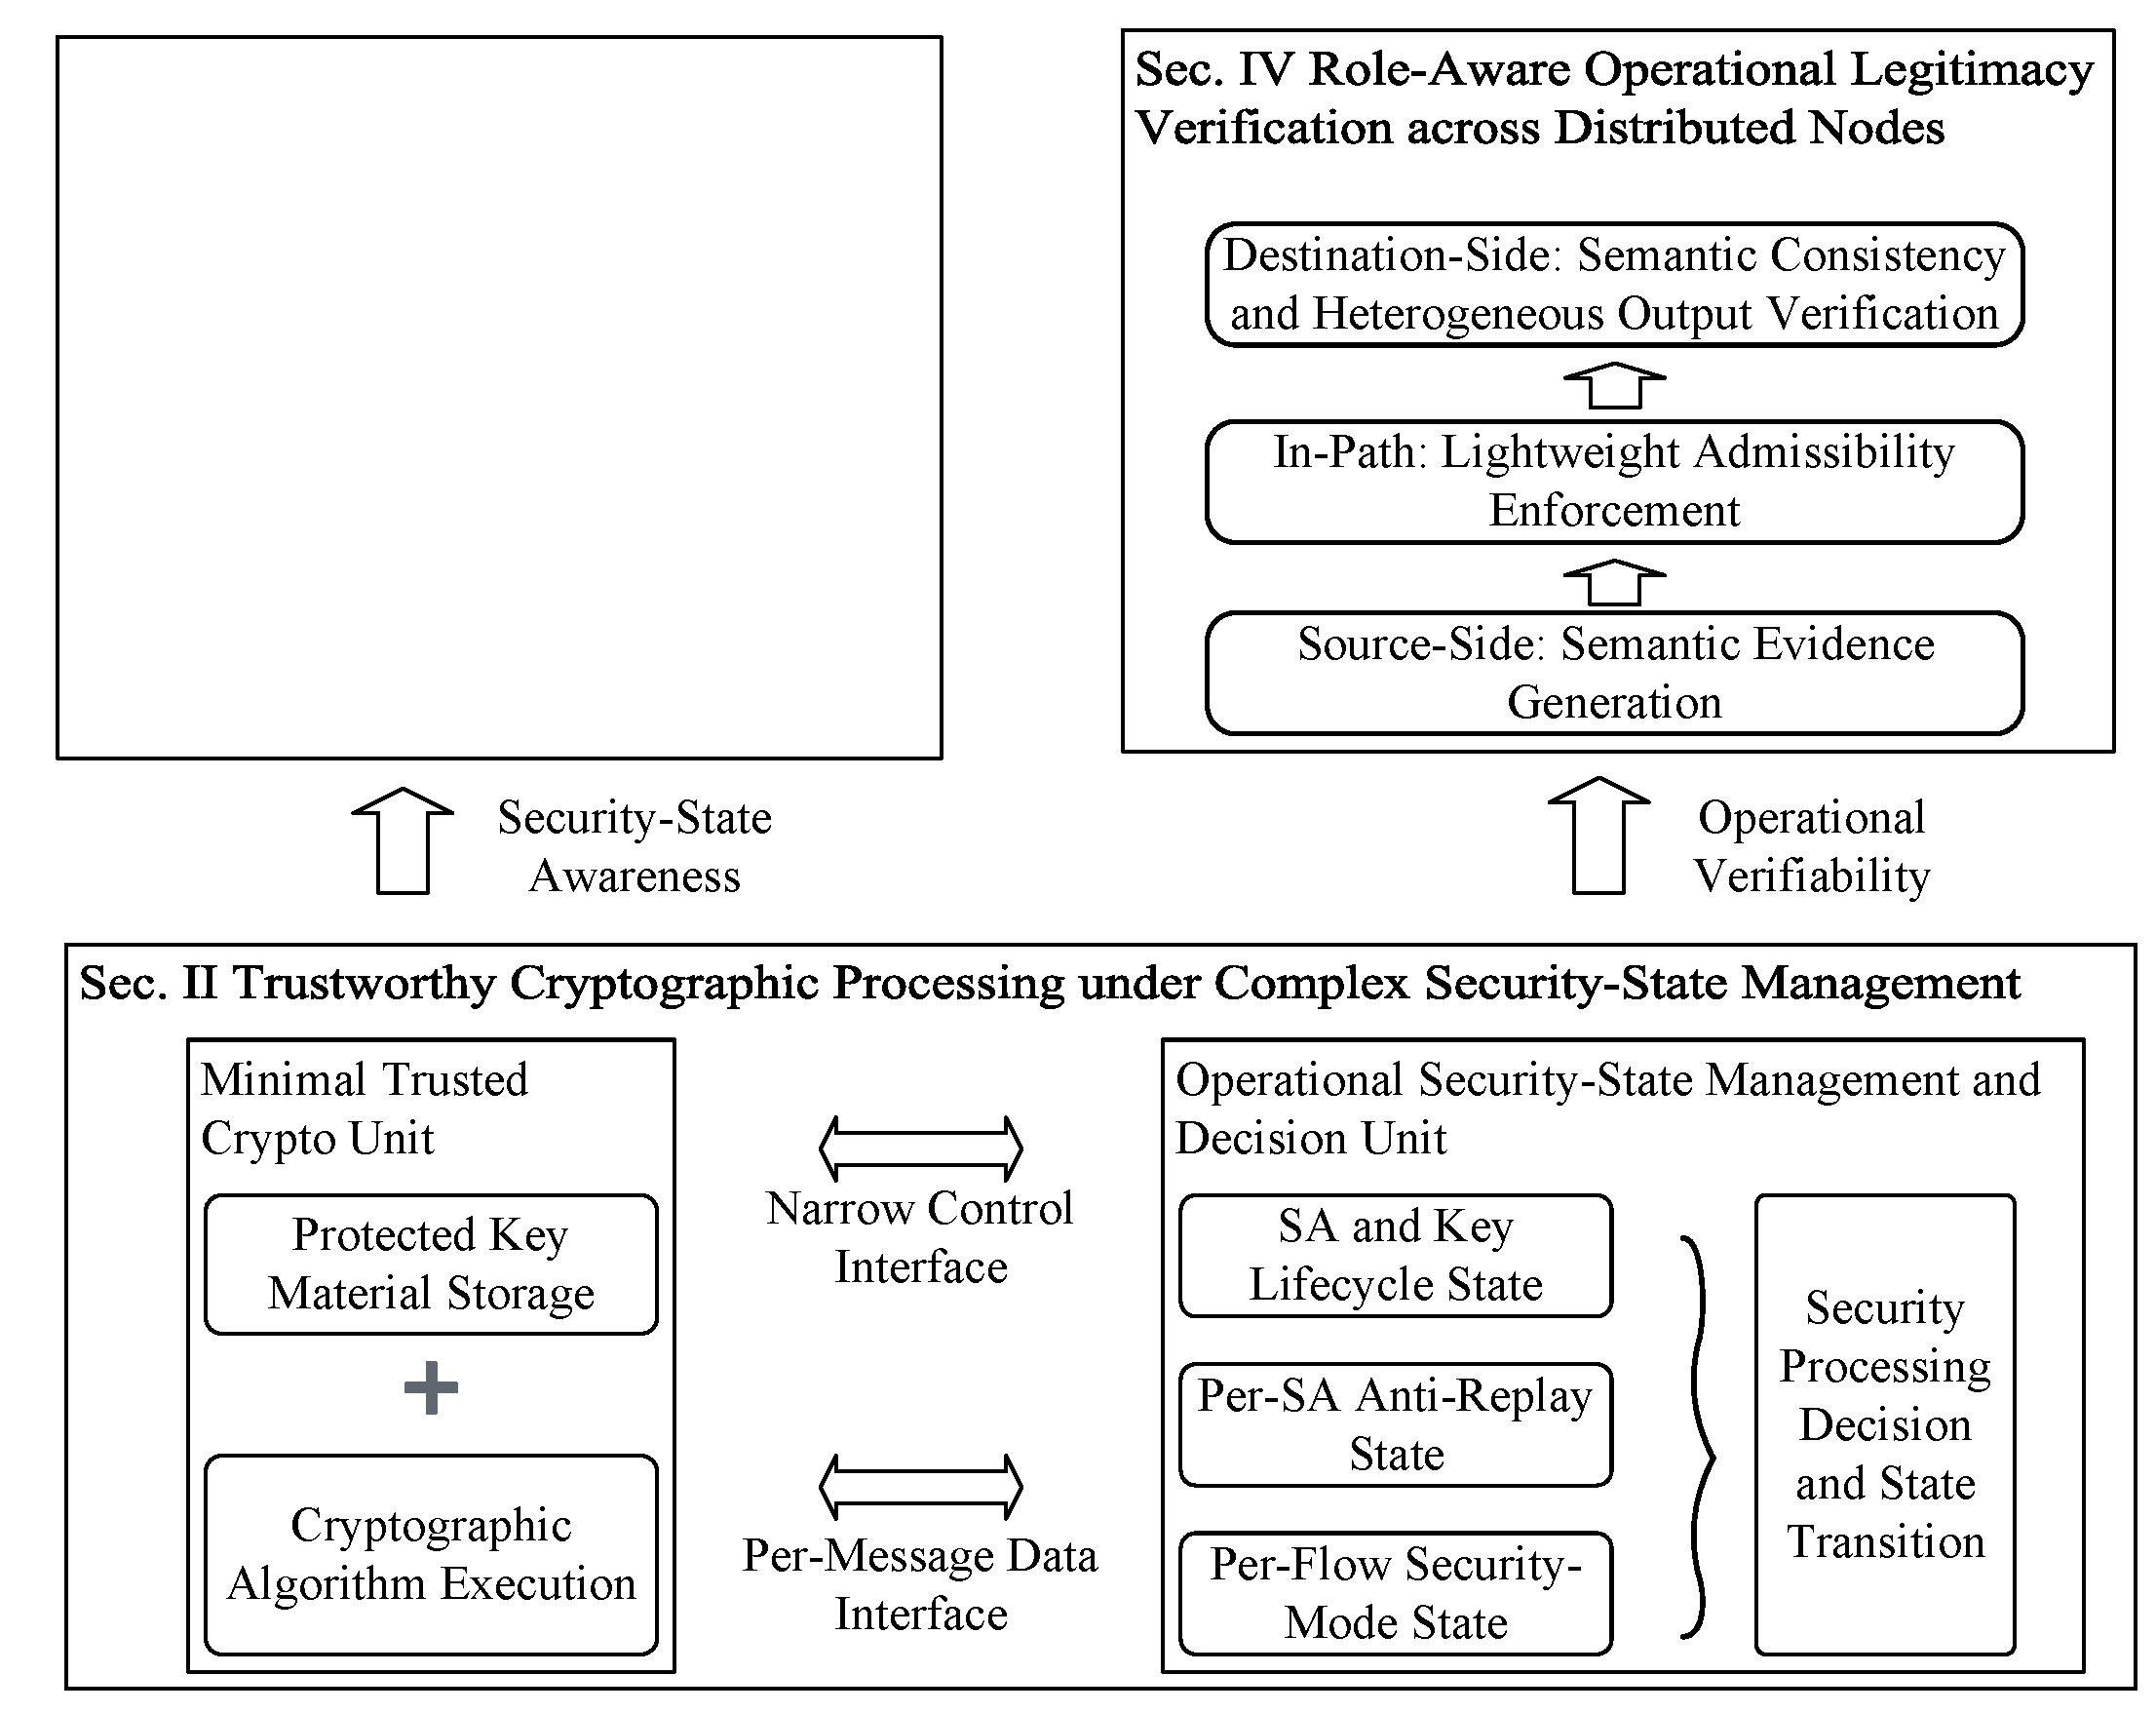
\includegraphics[width=1 \columnwidth]{figure/PaperStructureV2.pdf}
\caption{ 
XXXX
}
\label{fig:PaperStructure}
\end{figure}


\section{Trustworthy Cryptographic Processing under Complex Security-State Management} 
\label{sec:point1}

\subsection{Security-State Complexity and Design Principles} 
\label{subsec:point1-Drivers}
The complexity of onboard security-state management is increasing along three closely coupled dimensions. 
% 先从以下3点论证系统状态复杂性提升
% 1. 单流到同时管理多流、且每个流都包含各自的明密状态。
% 2. 多流可以使用相同或不同的密钥，导致需要管理多对1的映射关系。
% 3. 从预置密钥池演化到支持空中更新密钥，时间上涉及密钥生命周期管理的问题，空间上由于星地链路丢帧错帧，会涉及星地密钥同步问题。
First, modern satellites simultaneously carry heterogeneous traffic flows with different criticality and protection requirements, making per-flow security management preferable to a single link-wide configuration. Mission-critical flows such as telecommands can further support both protected and clear modes \cite{huang2026toward} to preserve essential functions in the event of onboard cryptographic failures. 
Second, each flow is associated with a corresponding Security Association (SA), while different SA may reference either distinct keys or a shared key. This creates nontrivial flow–SA–key dependency and mapping relationships, in which a change to one security object may affect multiple flows or processing contexts. 
Third, key management is evolving from the use of a statically preloaded key pool toward support for over-the-air key updates. This evolution introduces temporal complexity through key generation, activation, rollover, expiration, and revocation. It also introduces distributed-state consistency requirements, because the onboard and ground segments must maintain synchronized views of the active keys despite frame loss, transmission errors, delayed acknowledgments, and intermittent connectivity. 

%密码算法和密钥计算没有变复杂，但决定何时、以何种状态调用密码计算的管理逻辑越来越复杂。
Consequently, system complexity increasingly stems not from the cryptographic algorithms themselves, but from the evolving security states that govern when, where, and how cryptographic operations are invoked. 
% 这些新加入的复杂状态管理，会导致攻击面大大增大，而任何一点没做好，都会导致系统失效。比如攻击者可以通过破坏明密态、可以破坏流和密钥的映射关系、可以破坏星地密钥同步等。
This expanded state-management logic also enlarges the attack surface: an adversary may corrupt a flow’s clear/protected state, manipulate flow-to-key mappings, or disrupt key synchronization between the satellite and ground segments, causing legitimate traffic to be rejected or unauthorized operations to be accepted. 
These observations motivate the following two design principles. 

\begin{principle}[\textbf{Keep the Cryptographic Core Small}]
\label{principle:1}
Security-state management should be decoupled from cryptographic execution, leaving only key-dependent functions within a minimal and tightly controlled cryptographic boundary.
\end{principle}

\begin{principle}[\textbf{Low-Cost Checks First, Reject Early}]
\label{principle:2}
Security checks should proceed from simple, key-independent checks to costly cryptographic operations, enabling early rejection of invalid requests and reducing denial-of-service risks.
\end{principle}

The following Subsections \ref{subsec:point1-DecoupledStructure} and \ref{subsec:point1-ProcessingOrder} present a decoupled architecture and a progressive security-processing order based on these principles. 

\subsection{Decoupled Architecture with Controlled Interfaces}
\label{subsec:point1-DecoupledStructure}

CCSDS \cite{ccsds2022sdls} provides a well-established precedent for the first principle by managing Security Associations (SAs) and cryptographic keys through separate but coordinated lifecycles.
An SA transitions through \textit{Null, Unkeyed, Keyed, and Operational} states, whereas a key independently transitions through \textit{Pre-Activation, Active, Deactivated, and Destroyed} states.
The two are associated through the \textit{Rekey SA} procedure.

Building on this established separation, we broaden the managed state space beyond SA and key lifecycles.
This broader state space requires the trusted boundary to be redrawn between operational state management and cryptographic execution. 
As illustrated at the bottom of Fig. \ref{fig:PaperStructure}, the proposed architecture comprises a Minimal Trusted Cryptographic (MTC) unit and an Operational Security-State Management and Decision (OSMD) unit.
The MTC unit is limited to protected key-material storage and cryptographic algorithm execution, with its executable logic fixed before launch and not reconfigurable in orbit.
The OSMD unit, by contrast, maintains all operational security states, including per-flow security-mode states, per-SA anti-replay states, and the lifecycle states of SAs and keys.
It is also responsible for security-processing decisions, with reconfigurable logic that can be updated in orbit to accommodate evolving operational requirements and attack strategies.

All external requests terminate at the OSMD unit, leaving the MTC unit unexposed to other onboard or ground entities.
The OSMD unit receives space--ground messages, validates them against the current operational security states, and determines how they should be processed under satellite-specific constraints.
In particular, its processing order accounts for limited size, weight, and power (SWaP) resources and the resulting susceptibility to denial-of-service attacks, as discussed in Subsection \ref{subsec:point1-ProcessingOrder}.

The OSMD and MTC units interact through two narrowly defined internal interfaces.
The first is a control interface that supports only operations directly involving cryptographic key material.
For a symmetric-key implementation, operational keys are derived within the MTC unit from preloaded root keys and are securely deleted when no longer needed.
All other key-lifecycle states and decisions, such as activation and deactivation, remain within the OSMD unit and are not perceived by the MTC unit.
For example, deactivating a key only marks it as ineligible for subsequent use in the OSMD unit, whereas destroying the key additionally triggers its secure deletion from the MTC unit.
Accordingly, the control interface carries only simple commands such as $(\mathit{ParentKeyID}, \mathit{Derive}, \mathit{DerivedKeyID}, \mathit{Parameters})$ and $(\mathit{KeyID}, \mathit{Delete})$, and returns only an execution status.
No secret key material is transferred across this interface.

The second is a per-message data interface through which the OSMD unit requests cryptographic execution from the MTC unit.
Each request contains the original message, the requested cryptographic service, the selected key identifier, and any operation-specific parameters.
The MTC unit returns only the processed message and an execution status.
Thus, the interface exposes cryptographic execution as a narrowly defined service while keeping all state interpretation and security decisions within the OSMD unit.

The above interface definitions provide a concrete symmetric-key implementation of the proposed architecture.
Asymmetric cryptography can be supported by adding a small number of control operations, such as key-pair generation and shared-key establishment.
The generated private key and shared secret remain within the MTC unit, while only public keys and execution status are returned to the OSMD unit.
Therefore, supporting asymmetric cryptography does not alter the decoupled architecture or its minimal-interface principle; it only extends the set of cryptographic operations exposed through the controlled interface.


\subsection{Dependency-Aware Security Processing}
\label{subsec:point1-ProcessingOrder}

%总述
Consistent with Principle \ref{principle:2}, Fig. \ref{fig:point1} illustrates a progressive processing order across the OSMD and MTC units. 
The OSMD unit first performs lightweight, key-independent checks and invokes the MTC unit only after all applicable pre-cryptographic checks have succeeded.
Persistent security states are modified only on the basis of cryptographically authenticated inputs.
This ordering enables early rejection of invalid frames, conserves scarce onboard cryptographic resources, and prevents unauthenticated inputs from corrupting persistent security states.

\begin{figure}[t]
\centering
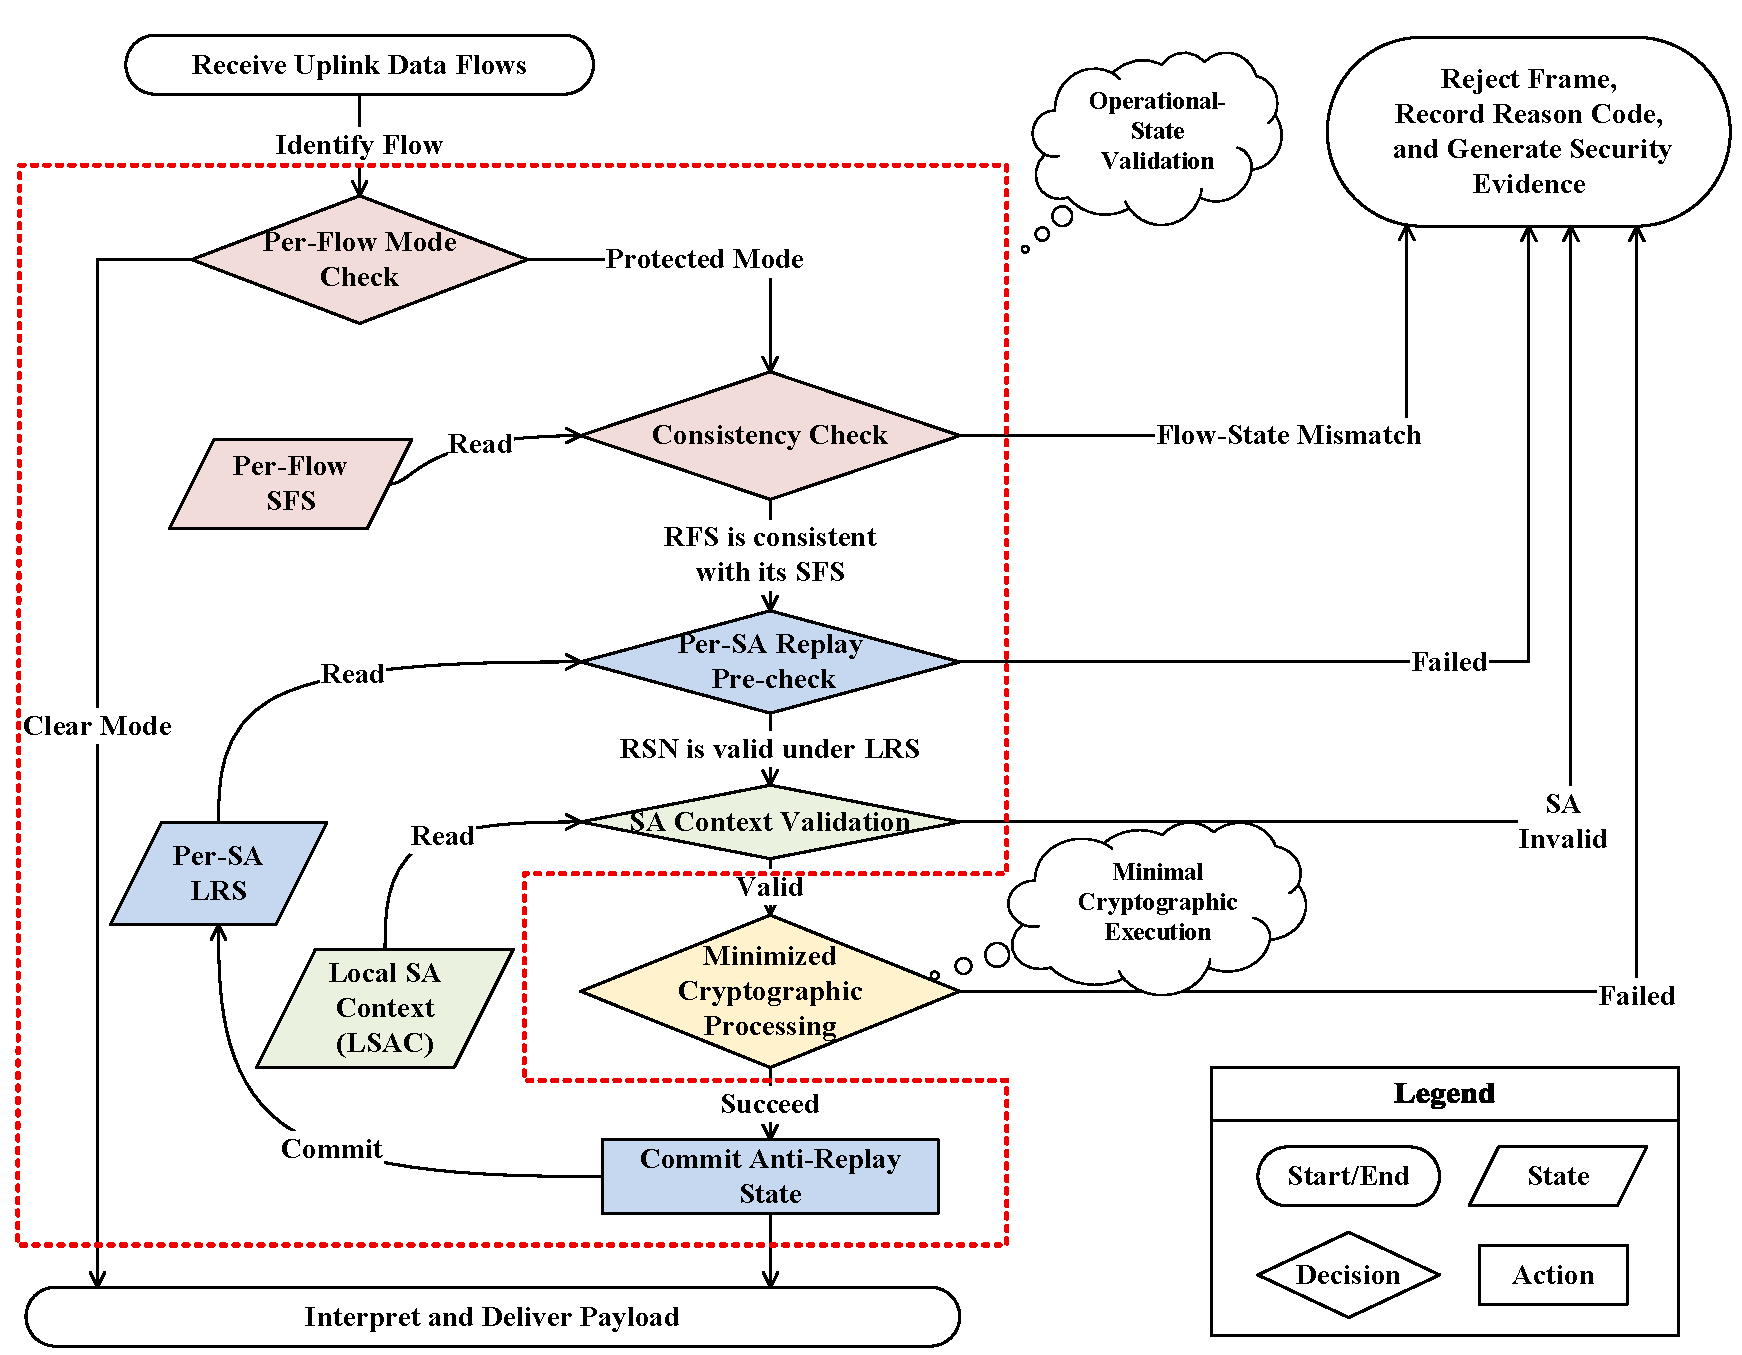
\includegraphics[width=\columnwidth]{figure/Point1V1.pdf}
\caption{Dependency-aware progressive processing across the OSMD and MTC units. The outer and inner red dashed boundaries delineate their respective processing scopes.}
\label{fig:point1}
\end{figure}

The processing begins with per-flow protection-state validation.
For each identified data flow, the OSMD unit maintains an authoritative \textit{System-Side Flow State} (SFS), which specifies whether the flow is currently required to operate in clear or protected mode.
Each received frame presents a corresponding \textit{Received Flow State} (RFS) through its actual protection format.
The OSMD unit proceeds only when the RFS is consistent with the SFS; otherwise, the frame is rejected before any SA processing or cryptographic operation is performed.

For a protected flow, each received frame carries a \textit{Received SA Identifier} (RSAI), indicating the Security Association (SA) under which it claims to be protected.
The RSAI is treated only as an untrusted reference and is used to locate the corresponding \textit{Local SA Context} (LSAC), which is authoritatively maintained by the OSMD unit.
The LSAC determines whether the claimed SA and its associated cryptographic resources remain authorized for use.
For example, an RSAI may reference an existing SA, while the key associated with that SA has already expired according to the locally maintained lifecycle state.
In this case, the OSMD unit rejects the frame without invoking the MTC unit.
Thus, the RSAI identifies the SA claimed by the incoming frame, whereas the LSAC determines whether that SA remains locally valid and operationally usable.

Once the RSAI has been resolved to an existing LSAC, the OSMD unit performs a lightweight anti-replay pre-check.
We distinguish the \textit{Received Sequence Number} (RSN), carried in the incoming frame, from the \textit{Local Replay State} (LRS), which is maintained locally for the referenced SA.

CCSDS SDLS provides the baseline anti-replay mechanism.
The receiver first verifies the integrity of a protected frame and then compares the authenticated RSN with the corresponding LRS.
The LRS is updated only after both checks have succeeded \cite{ccsds2022sdls}.
This ordering prevents an unauthenticated RSN from modifying the persistent replay state.
Otherwise, an attacker could inject a sufficiently large sequence number and cause subsequent legitimate frames to be rejected, resulting in a persistent denial-of-service condition.
However, the baseline ordering also requires every received frame, including an evident replay, to consume cryptographic processing time and energy.
Such overhead is particularly undesirable for onboard platforms subject to stringent size, weight, and power (SWaP) constraints.

To reduce this overhead, we introduce a two-stage replay check inspired by IPsec ESP \cite{kent2005security4303}.
Before cryptographic verification, the OSMD unit compares the unauthenticated RSN with the current LRS.
Frames that are evidently stale or lie outside the configured admissible advance range are rejected without invoking the MTC unit.
Because the RSN has not yet been authenticated, this pre-check serves only as an early filter and cannot modify the LRS.

Frames passing the replay pre-check then undergo full LSAC validation.
Only frames associated with a valid and authorized SA context are forwarded to the MTC unit for cryptographic processing.
After successful cryptographic authentication, the OSMD unit performs the definitive replay check using the authenticated RSN and the current LRS.
The LRS is updated to incorporate the RSN only if this final check succeeds.
Consequently, the pre-check reduces unnecessary cryptographic operations, while the authenticated post-check remains the sole authority for committing replay-state transitions.

Overall, each processing stage relies only on information established by the preceding stages.
The admissible frame set is progressively narrowed before cryptographic execution, while persistent state transitions are postponed until the corresponding inputs have been authenticated.



\section{Constrained Security-State Perception and Reconstruction} 
\label{sec:point2}
% 本段承接上一节的星上可信状态管理，指出“状态可信”并不等于“地面能够可靠感知状态”。
% 随后概括敏感信息不可直接披露和星地回传资源有限两项核心约束，并引出由状态定义、证据转换和渐进重构组成的三阶段逻辑。
Section~II has established trustworthy onboard management of complex security states. However, a trustworthy state-management process does not automatically make its evolving state reliably perceivable to the ground.
The relevant state may span a flow's clear/protected mode, Security Association (SA) and key lifecycles, policy and route versions, and the current boot instance. 
Moreover, there are two satellite-specific constraints.  
Some raw states and their temporal correlations are too sensitive to disclose, while intermittent and capacity-limited return links cannot carry all admissible evidence in real time. 
The upper-left block of Fig.~1 therefore follows a three-stage logic: define what the ground must distinguish, transform sensitive state into disclosure-safe evidence, and prioritize that evidence for progressive reconstruction. 

\subsection{Flow-Centric Security-State Semantics}
% 本段说明现有机制分散管理平台、SA、密钥、策略和路由对象，单个对象各自合法仍不足以保证业务流受到连续保护。
% 为弥合这一状态断层，本文以持续业务流标识绑定各类对象，并从局部合法性、路径一致性和转换连续性三个层面定义安全属性。
Existing mechanisms usually manage platform integrity, SAs, keys, policies, and forwarding entries as separate objects. Their local validity is necessary but insufficient. 
For example, an SA may be active but associated with an obsolete route epoch, or traffic may migrate before every node on the new path has activated a compatible protection context. We therefore bind these objects to a persistent service-flow identity and distinguish three property classes.

- \emph{\textbf{Local admissibility}} requires an authorized policy, usable SA, and non-revoked key. 

- \emph{\textbf{Path consistency}} requires participating nodes to use compatible flow and protection contexts. 

- \emph{\textbf{Transition continuity}} constrains their ordering during migration, rekeying, policy replacement, and reset recovery.

% 本段利用路径迁移和卫星复位两个典型事件，说明上述安全属性如何落到时间顺序与上下文约束上。
% 重点不是收集完整日志，而是提取能够区分安全与不安全演化的关键状态关系、边界事件及其依赖结构。
Consider a flow moving from an old path to a new one.
New-path protection must become ready before traffic migration, whereas old-path protection must remain valid until migration is complete. 
Evidence generated across a reset must additionally carry a trustworthy boot epoch; otherwise, an obsolete pre-reset state could be mistaken for a valid continuation.
The output is therefore not a complete log, but a property-dependency model identifying the state relations and boundary events needed to distinguish safe from unsafe evolution.

\subsection{Disclosure-Safe Evidence and Sound Reconstruction}

% 本段界定披露约束的范围。需要保护的不仅是SA标识、密钥周期等单项状态值，还包括时间戳和跨节点关联可能暴露的任务活动，因此证据设计必须同时控制字段披露与关系披露。
Directly reporting SA identifiers, key epochs, detailed policies, route changes, or mission modes may expose sensitive operations.
Hiding individual fields is also insufficient when timestamps and cross-node correlations reveal the concealed activity.
The disclosure boundary must consequently cover both state values and their relationships.

% 本段提出由星上可信功能将原始状态转换为受限范围内的属性声明，并列举可采用的证据形式。
% 远程证明和受限披露研究用于说明可信证据框架及隐私保护手段已有基础；
% 本文真正需要解决的是，哪些业务流级谓词足以支持地面对跨对象、跨路径和跨时间安全关系作出判断。
A trusted onboard evidence function converts raw state into scoped property claims. Depending on mission policy and onboard capability, these may be signed assertions, authenticated interval summaries, commitments with membership proofs, or zero-knowledge proofs.
Remote attestation already provides a hardware-rooted evidence--verification architecture \cite{rfc9334rats}, and constrained-disclosure attestation demonstrates that selected properties can be verified without releasing complete measurements \cite{eckel2023racd}.
The unresolved design issue is which flow-level predicates are sufficient. Proving that an SA is active, for example, is weaker than proving that it is compatible with the current flow and route epoch and became active before migration.

% 本段给出每项证据声明必须携带的上下文，并说明地面如何依据状态模型和已接收证据维护候选演化集合。
% Verified、Violated 和 Indeterminate三值结论体现保守验证原则：
% 缺失或隐藏信息只能降低结论完备性，不能被默认解释为系统安全。
Each claim must therefore be scoped by a controlled flow identifier, node or role, boot and route contexts, validity interval, asserted property, provenance, freshness, and authenticator.
The ground then maintains the set of security-state evolutions consistent with the model and all received claims.
A flow is \emph{Verified} only if every remaining evolution satisfies the target property, and \emph{Violated} if authenticated evidence establishes its violation. 
If safe and unsafe evolutions both remain possible, the result is \emph{Indeterminate}.
This conservative semantics follows runtime verification under partial information \cite{leucker2019partial}: hidden or missing evidence reduces completeness, but must never weaken the meaning of a verified result.

\subsection{Resource-Aware Progressive Reconstruction}
% 本段明确资源调度位于披露策略之后，即只能从允许下传的证据中进行选择。
% DTN解决证据在间歇链路上的可靠送达，但本文进一步按照证据对当前验证结论的边际贡献排序，并综合考虑传输、计算、能耗、时效和依赖成本。
Resource constraints are applied only after the disclosure policy has determined which evidence forms are admissible. Delay-tolerant networking can reliably carry evidence across disrupted contacts \cite{rfc9171bpv7}, but it does not decide what deserves scarce return-link capacity. Evidence should instead be prioritized by its marginal contribution to the current verdict.
Repeated steady-state reports may add little, whereas one authenticated transition claim may eliminate the last unsafe candidate evolution. Its value should be weighed against transmission size, generation cost, energy, expiration time, and dependencies on other claims.

% 本段描述渐进重构的闭环机制。
% 为支持按需下传，关键检查点和状态转换证据应能够独立验证；每批证据用于收缩候选演化集合。
% 若结论仍不确定，地面便定位最小歧义并发起属性级定向补证，同时校验证据所属的来源与重构上下文。
This selection requires independently verifiable checkpoints and transition claims rather than a cumulative log that can be validated only in full. Reconstruction then becomes a closed loop.
Each received batch removes incompatible candidate evolutions. If the verdict remains \emph{Indeterminate}, the ground identifies the smallest unresolved relation and requests evidence scoped to a flow, node or role, epoch, interval, and property.
Out-of-order evidence is accepted only after its provenance and context match the reconstruction instance.

% 本段用路径迁移案例串联前述三层设计，说明缺失一项新路径就绪证据时必须保持Indeterminate，并仅请求能够消除该歧义的属性。
% 案例强调资源不足可以延迟结论，却不能降低 Verified 的证据门槛；段末同时衔接下一节的运行合法性验证。
In the migration example, suppose the first contact reports the migration and old-path withdrawal but omits one new-path readiness claim.
The ground must retain an \emph{Indeterminate} verdict and request only that missing property. A later claim either establishes continuous protection
or exposes a transition gap.
Thus, limited resources may delay a conclusion, but cannot lower the evidentiary threshold for \emph{Verified}. The resulting scoped verdicts provide Section~IV
with reliable security knowledge for role-aware operational-legitimacy verification. 


\section{Role-Aware Distributed Verification of Operational Legitimacy}
\label{sec:point3}

The preceding two sections establish a trustworthy cryptographic foundation under complex security-state management and enable the ground segment to reliably perceive onboard security states, respectively. Building on this foundation, this section takes the next step toward operational legitimacy through system-level verification that actively generates and coordinates evidence across the system. 

In future networked satellite systems with onboard routing and processing, a security-critical operation may traverse multiple nodes and processing stages before being ultimately executed. As illustrated in Fig. \ref{fig:point3}, we abstract this process into three node roles: source, transit, and destination. Because these roles have access to different information and support different defensive actions, we develop three complementary verification mechanisms tailored to their respective capabilities in Subsections \ref{subsection:ponit3-1sourceDestination}, \ref{subsection:ponit3-2transit}, and \ref{subsection:ponit3-3Destination}.

\begin{figure}[h]
\centering
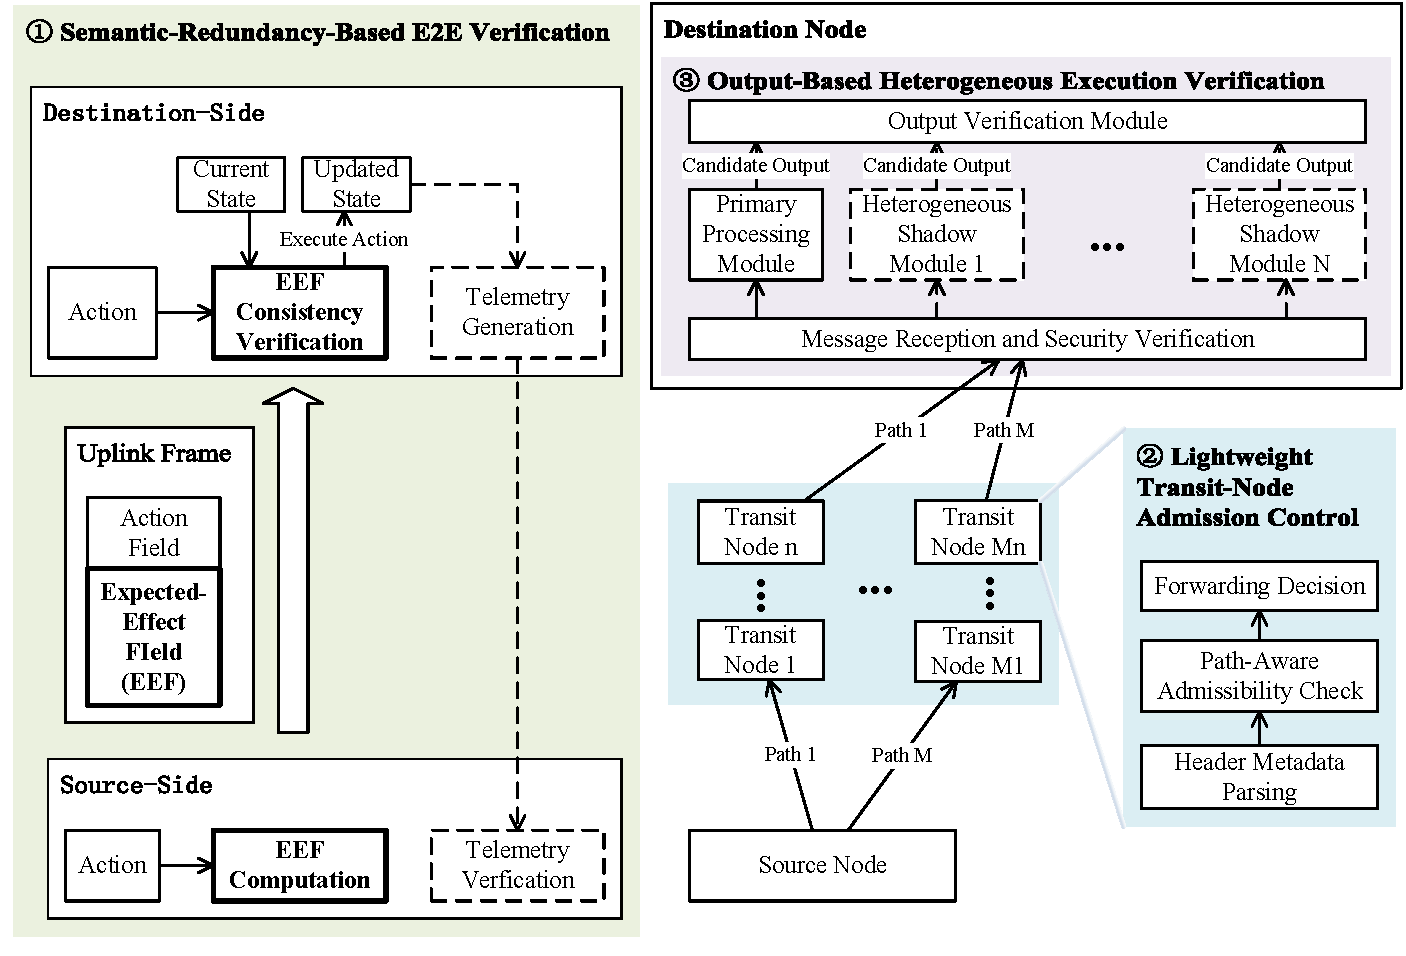
\includegraphics[width=1 \columnwidth]{figure/Point3V3.pdf}
\caption{Role-aware distributed verification of operational legitimacy across the source, transit, and destination nodes along the message-processing chain. 
The green, blue, and purple blocks represent three complementary mechanisms for verifying action-effect consistency between the endpoints, path admissibility at transit nodes, and execution consistency at the destination node, respectively.}
\label{fig:point3}
\end{figure}


\subsection{Semantic-Redundancy-Based End-to-End Verification}
\label{subsection:ponit3-1sourceDestination}
%本段的核心思路
The first mechanism is motivated by the insight that the source node can determine the expected effect of a command when it is correctly executed by the destination node. 

%现状

As indicated by the dashed lines in the green block of Fig. \ref{fig:point3}, conventional end-to-end verification of command effects is largely ground-centric and retrospective, typically relying on telemetry returned after onboard execution \cite{ecss7031c}. 
The destination node first executes the action carried in the uplink frame, after which the resulting state change is reported through telemetry. The source node can therefore complete the verification only after receiving the corresponding telemetry, potentially introducing substantial delay when constrained space-to-ground bandwidth permits the relevant state to be downlinked only at a low cadence. 

%改进方法：引入语义冗余
To this end, we add an Expected Effect Field (EEF) to the uplink frame as a ``semantic checksum'' for pre-execution verification. As highlighted by the bold-outlined components in the green block of Fig. \ref{fig:point3}, the source node derives the EEF from the intended action and its locally maintained state, then embeds it in the frame. Upon reception, the destination node independently recomputes the EEF using the received action and its current state. The action is executed only when the two EEF values match. 

%机理和效果
By introducing semantic redundancy, the EEF enables real-time end-to-end verification before onboard action execution. 
As illustrated in the following example, it can detect two classes of inconsistency: unexpected alterations to the onboard state and incorrectly encoded actions, thereby preventing unintended execution.


\begin{example}[\textbf{Power-Level Adjustment}]
Consider an onboard transmitter with discrete power levels and two actions that increase or decrease the current level by one. 

If the source node believes that the current level is $k$ and issues an increase action, it sets the EEF to $k+1$.
The destination node independently derives the expected post-action level from the received action and its actual state, executing the action only if the result matches the EEF.

A mismatch therefore exposes either an unexpected change in the onboard state (e.g., malicious alteration or a reboot-induced reset) or an incorrectly encoded action (e.g., a decrease in place of the intended increase).
In either case, the action is rejected before execution.
\end{example}

\subsection{Lightweight Transit-Node Admission Control}
\label{subsection:ponit3-2transit}

Transit nodes typically inspect only the header fields required for forwarding.
Given their SWaP constraints and the high aggregate volume of multi-flow traffic, payload inspection or full-fledged IDS at every transit node is impractical and largely redundant with destination-side detection.

As shown by the blue block in Fig. \ref{fig:point3}, we instead enable transit nodes to perform lightweight admission control using compact, integrity-protected header metadata identifying the source, destination, and message type.
Each transit node combines this metadata with its local path context to determine whether the traffic is admissible from its position in the forwarding path.

Consider the attack described in the introduction, in which a compromised user terminal injects a well-formed and cryptographically valid TT\&C message.
The first-hop onboard router observes that the message enters from the user-access domain and is classified as TT\&C traffic.
Because this domain is not authorized to originate such traffic, the router rejects the frame before forwarding.

Such early filtering is important because ingress provenance and other path-specific context may be lost or obscured after forwarding.
Detecting the same violation at downstream nodes may therefore require substantially more expensive payload inspection or intrusion detection.
A small amount of additional header metadata thus enables low-cost suppression of inadmissible traffic close to its point of entry.

Existing mechanisms provide partial foundations for this design.
IEEE 802.1Qci \cite{ieee8021qci} establishes an engineering baseline for lightweight forwarding-plane enforcement through Per-Stream Filtering and Policing (PSFP), whereas our mechanism extends such enforcement from traffic conformance to operational admissibility.
Similarly, RFC 3704 \cite{rfc3704} specifies ingress filtering and unicast Reverse Path Forwarding (uRPF) to assess whether a packet arrives from a direction consistent with its claimed source address.
Our mechanism goes beyond source plausibility by further verifying whether the claimed source is authorized to originate the claimed message type.

\subsection{Output-Based Heterogeneous Execution Verification}
\label{subsection:ponit3-3Destination}

At the destination node, where an operation is ultimately executed, additional computational resources can be deliberately introduced to strengthen the assurance of security-critical operations.

Unlike the end-to-end mechanism in Subsection \ref{subsection:ponit3-1sourceDestination}, which primarily verifies the consistency of the \textit{states} maintained by the source and destination nodes, the mechanism proposed here focuses on the consistency of \textit{execution outputs}.
Directly comparing all internal states is often impractical in a complex system because the relevant states may be numerous, implementation-specific, or security-sensitive.
In particular, some states, such as cryptographic keys or key-related identifiers, should remain confined within their respective hardware or trusted processing boundaries.
We therefore verify execution consistency through externally observable outputs rather than through direct exposure or comparison of internal states.

As shown in the purple block of Fig. \ref{fig:point3}, the primary processing module is supplemented with one or more heterogeneous shadow modules.
An incoming message first passes through the message authentication module, which performs the cryptographic checks described in Section \ref{sec:point1} and the end-to-end semantic verification introduced in Subsection \ref{subsection:ponit3-1sourceDestination}.
Only messages that pass these checks are dispatched simultaneously to the primary processing module and the shadow modules.
Each module processes the same authenticated input independently, and their outputs are forwarded to an output verification module.
The operation is accepted only when the resulting outputs satisfy a predefined consistency rule; otherwise, execution is blocked, deferred, or reported as anomalous.

The use of heterogeneous implementations is essential to reducing common-mode compromise.
Although redundant or backup processing units are widely employed in satellite systems, homogeneous replicas may share the same hardware vulnerabilities, software defects, or exploitable implementation assumptions.
We therefore advocate implementing the shadow modules using diverse hardware architectures, software stacks, or processing paradigms, so that a single attack or fault is less likely to induce the same erroneous output across all modules.
For example, the primary and shadow modules may employ different CPU architectures, while an additional shadow implementation may be realized on an FPGA.
Such diversity allows output agreement to provide stronger evidence of correct execution than conventional homogeneous redundancy.




\section{Case Study}
%混合攻击场景
%这里重要的是展示对多类攻击的多层级过滤；先过滤dos，可以基于帧格式、mode错误等，然后再对抗重放攻击。
attacks with wrong clear mode

attack with 

\section{Conclusion}
\label{sec:conclusion}

1. a decoupling structure instructed by principles. 
2. XXX
3. a systematic solution that let every component at different position to contribute their own effect. 


\bibliographystyle{IEEEtran}
\bibliography{RSE}


% that's all folks
\end{document}


